\section{Hardware Interfaces}

Hardware interfaces are implemented as plugins that follow a 
lifecycle model similar to ROS2 Lifecycle Nodes. 
This design allows for better management of hardware 
resources and more robust error handling.


\subsection{Hardware Interface Lifecycle}

The lifecycle of a Hardware Interface in ROS2 Control consists of several states:

\begin{enumerate}
    \item Unconfigured
    \item Inactive
    \item Active
    \item Finalized
\end{enumerate}


\begin{figure}[ht]
    \centering
    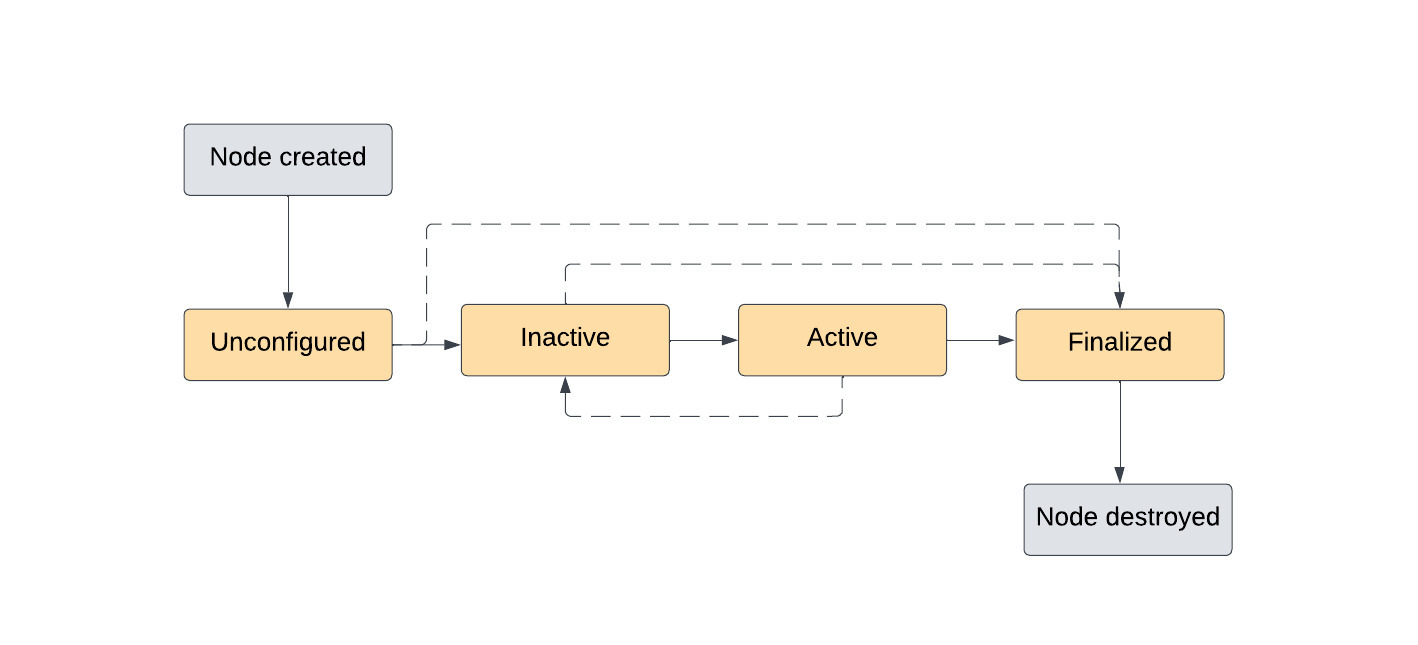
\includegraphics[width=0.9\textwidth]{Live_Nodes_OverView.jpeg}
    \caption{ROS2 Live Node Overview}
    \label{fig:mesh4}
\end{figure}

Each state transition triggers specific callback functions.

\begin{figure}[ht]
    \centering
    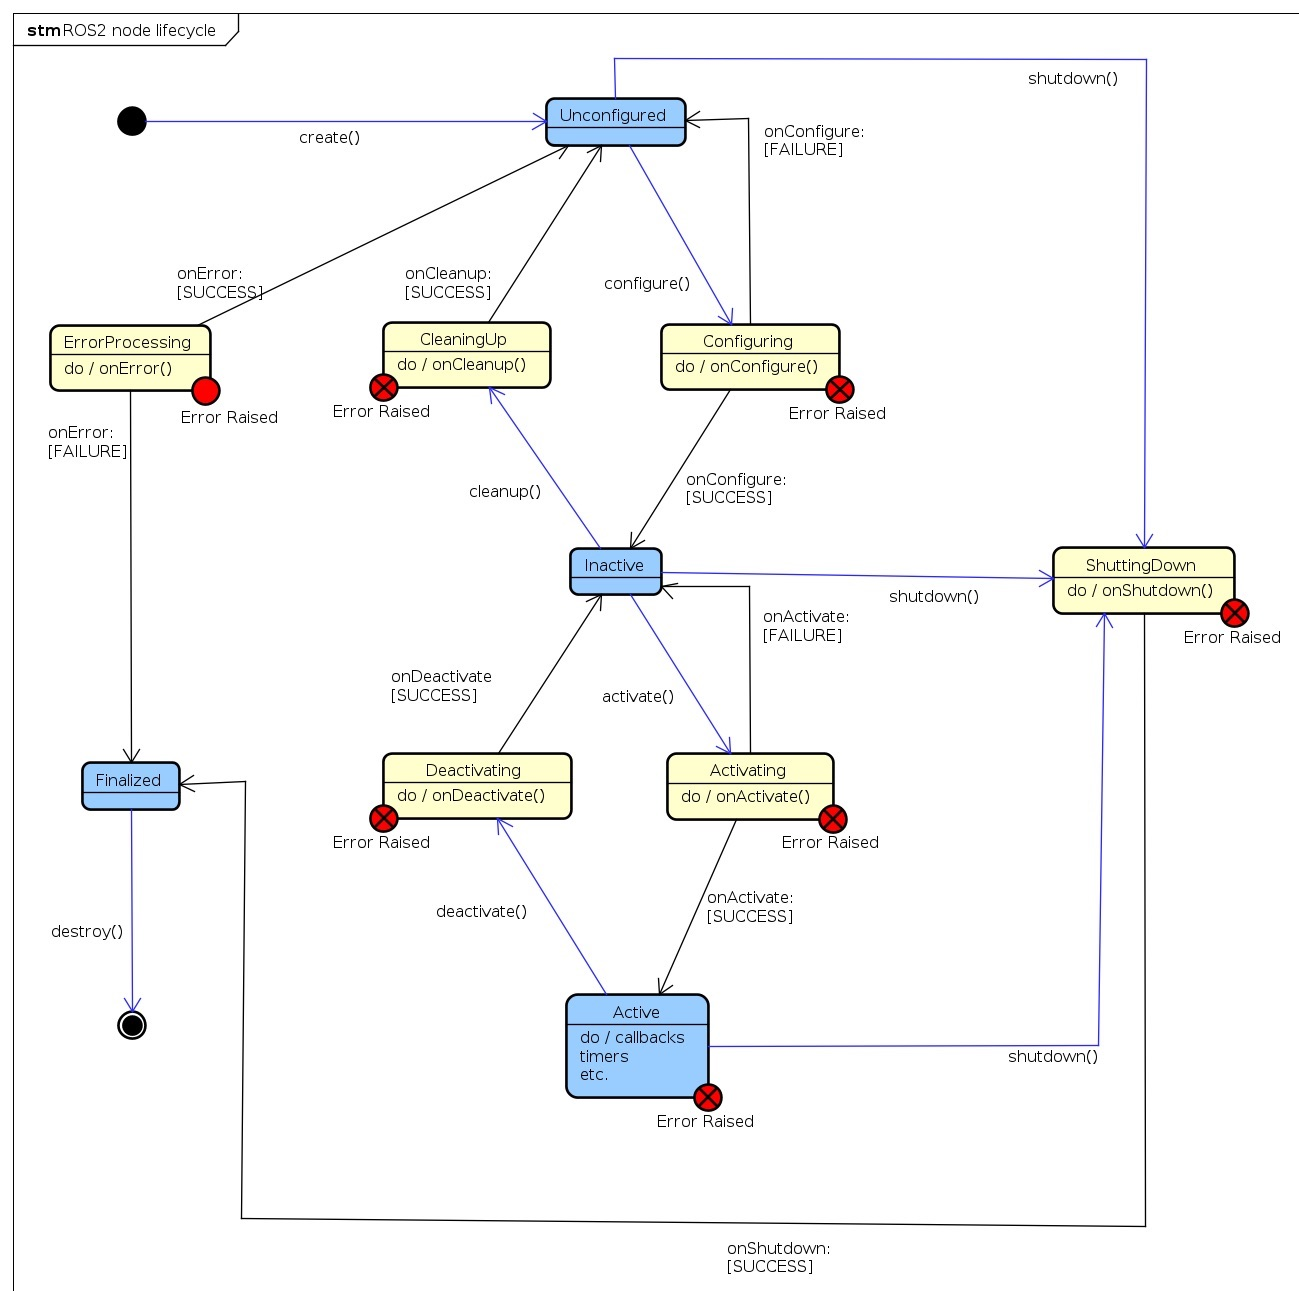
\includegraphics[width=0.9\textwidth]{Live_Nodes_State_Machine.jpeg}
    \caption{ROS2 Live Node State Machine}
    \label{fig:mesh5}
\end{figure}

\begin{itemize}
    \item \texttt{on\_init()}: Called when initializing the hardware interface
    \item \texttt{on\_configure()}: Sets up communication with the hardware
    \item \texttt{on\_activate()}: Prepares the hardware for operation
    \item \texttt{on\_deactivate()}: Stops hardware operation
    \item \texttt{on\_cleanup()}: Cleans up resources
    \item \texttt{on\_shutdown()}: Prepares for shutdown
    \item \texttt{on\_error()}: Handles errors during operation
\end{itemize}

\subsection{Asynchronous Communication}

synchronous communication is crucial for Hardware Interfaces, especially when dealing with real-time control systems or hardware with varying response times.
Since KUKAVARPROXY uses TCP, you'll need to implement asynchronous communication to avoid blocking the control loop.

\begin{enumerate}
    \item \textbf{Non-blocking operations}: Asynchronous communication allows the control loop to continue running without waiting for hardware responses, maintaining system responsiveness.
    
    \item \textbf{Handling slow hardware}: Some hardware components may have slow update rates or communication delays. Asynchronous operations prevent these delays from affecting the entire control system.
    
    \item \textbf{Parallel processing}: Multiple hardware components can be read from or written to simultaneously, improving overall system performance.
    
    \item \textbf{Error resilience}: Asynchronous operations can better handle timeouts and communication errors without blocking the entire system.
\end{enumerate}
